\documentclass{article}

\usepackage{listings}
\usepackage{xcolor}
\usepackage{graphicx}
\usepackage{caption}

% Define colors for code listing
\definecolor{codegreen}{rgb}{0.1,0.5,0.1}
\definecolor{codegray}{rgb}{0.5,0.5,0.5}
\definecolor{codepurple}{rgb}{0.5,0.0,0.3}
\definecolor{backcolour}{rgb}{0.95,0.95,0.92}

% Define code listing settings
\lstdefinestyle{mystyle}{
    backgroundcolor=\color{backcolour},
    commentstyle=\color{codegreen},
    keywordstyle=\color{codepurple},
    numberstyle=\tiny\color{codegray},
    stringstyle=\color{blue},
    basicstyle=\ttfamily\small,
    breakatwhitespace=false,
    breaklines=true,
    captionpos=b,
    keepspaces=true,
    numbers=left,
    numbersep=5pt,
    showspaces=false,
    showstringspaces=false,
    showtabs=false,
    tabsize=2
}

% Set code listing style
\lstset{style=mystyle}

\begin{document}

\title{Exploratory Data Analysis for The The Seattle Airbnb Dataset}
\author{Rabab Moubine}
\maketitle

\section{Brief description of the data set and a summary of its attributes}

The Seattle Airbnb data set contains information about the listings and reviews of Airbnb in Seattle, Washington. It consists of three files: listings, calendar, and reviews. \\
The listings file has 92 attributes, including property type, room type, neighbourhood, price, availability, number of reviews, and host information, the calendar file has information about the availability and price of each listing on a given data and the reviews file includes information about the guest reviews and ratings for each listing. \\
The listing file was the most pertinent for the project, and therefore, the only file used for analysis.

\section{Initial plan for data exploration}

The initial plan for data exploration is to first gain a general understanding of the data, including the size of the data set, the number of missing values, and the distribution of the attributes. Then, I will perform univariate and bivariate analysis to explore the relationships between different attributes. 
I will also create visualizations, such as histograms, scatterplots, and heatmaps, to help identify patterns and correlations in the data.                                                                                                   

\section{Actions taken for data cleaning and feature engineering}
\textbf{• Dropping non relevant features}\\
The following steps were taken for data cleaning and feature engineering:\\
Firstly, non-numerical features and irrelevant ones were dropped, such as 'listing\textunderscore url', 'source', 'name', 'description', 'neighbourhood\textunderscore overview', 'picture\textunderscore url', 'host\textunderscore url', etc. \\
Secondly, features representing IDs, namely 'id', 'scrape\textunderscore id', and 'host\textunderscore id', were dropped. \\
Lastly, the 'bathrooms' feature was dropped as it had no data and was empty.\vspace{.5cm}

\textbf{• Handling missing values}\\
\begin{lstlisting}[language=Python, caption=Python code snippet for missing values]
df.isnull().sum().sort_values(ascending=False)
\end{lstlisting} 
Missing values were identified in certain features, namely 'review\textunderscore scores\textunderscore value', 'review\textunderscore scores\textunderscore location', 'review\textunderscore scores\textunderscore accuracy', 'review\textunderscore scores\textunderscore checkin', 'review\textunderscore scores\textunderscore communication', 'review\textunderscore scores\textunderscore cleanliness', 'last\textunderscore review\textunderscore duration\textunderscore in\textunderscore days', 'first\textunderscore review\textunderscore duration\textunderscore in\textunderscore days', 'reviews\textunderscore per\textunderscore month', 'review\textunderscore scores\textunderscore rating', 'bedrooms', and 'beds'.\\
The missing values in the review scores and bedrooms features were replaced with the median due to skewed data. For the 'beds' feature, the 71 rows with missing values were removed.\vspace{.5cm}

\textbf{• Transforming data types}\\
In this dataset, many features were of object type, so I performed several transformations\\
For instance, I converted the features 'host\textunderscore is\textunderscore superhost', 'host\textunderscore has\textunderscore profile\textunderscore pic', 'host\textunderscore identity\textunderscore verified', 'has\textunderscore availability', and 'instant\textunderscore bookable' from string values of "t" and "f" to binary values of "1" and "0", respectively.\\
To transform the date features 'host\textunderscore since', 'first\textunderscore review', and 'last\textunderscore review', I calculated the duration until the dataset was last scraped using the 'last\textunderscore scraped' feature.\\
For the 'host\textunderscore location' feature, which had 162 unique locations, I simplified it by keeping only the four most frequent locations ['Seattle, WA', 'New York, NY', 'San Francisco, CA', 'Bellevue, WA'] and creating an 'Others' category for the remaining locations.\\
Moreover, I removed any non-numeric signs such as "\%" or "\$" from the values of 'host\textunderscore response\textunderscore rate', 'host\textunderscore acceptance\textunderscore rate', and 'price'.\\
Finally, I transformed the 'property\textunderscore type' feature into three categories: 'wholeUnit', 'room', and 'other'. The 'property\textunderscore type' feature was then one-hot encoded, and the original feature was dropped from the dataset.\vspace{.5cm}

\textbf{• Encoding categorical variables}\\
In the cleaning process of the Airbnb Seattle dataset, categorical features were encoded to numerical values to allow for better analysis and modeling. \\
The 'host\textunderscore location' column was filtered based on a list of preferred locations, and then one-hot encoded using Pandas' get\textunderscore dummies function.\\
The 'room\textunderscore type' column was also one-hot encoded and the 'Shared room' and 'Hotel room' categories were dropped. \\
The 'property\textunderscore type' column was transformed using a custom function and then one-hot encoded. 
The resulting encoded columns were concatenated with the original dataset and the original categorical columns were dropped.\\
These encoding techniques allowed for a more comprehensive analysis of the dataset and enabled machine learning models to be trained on the data.\vspace{.5cm}

\textbf{• Creating new features from existing ones}\\
In order to simplify the host verification feature, which had five possible values, including combinations of 'email', 'phone', and 'work\textunderscore email', I transformed it into three separate features: host\textunderscore verifications\textunderscore phone, host\textunderscore verifications\textunderscore email, and host\textunderscore verificationsv\textunderscore work\textunderscore email. For each new feature, a value of 1 was assigned if the corresponding verification method was present, and 0 if it was not.\\
The 'bathrooms\textunderscore text' feature, which contained textual descriptions of bathrooms, was transformed into a numerical feature called 'bathrooms\textunderscore number'.\\
The 'amenities' feature was transformed by counting the number of amenities listed. The resulting value was stored in a new feature called 'amenities\textunderscore number', and the original 'amenities' column was then dropped using the 'drop' method in pandas.\\
A new feature was created in the Airbnb Seattle dataset called 'distance\textunderscore from\textunderscore city\textunderscore center' by calculating the distance between the latitude and longitude of each listing and the central point of the city using the Haversine formula.\\
Finally, the original latitude and longitude columns were dropped from the dataset.\vspace{.5cm}

\textbf{• Removing outliers}\\
To gain insights into the data and identify any potential outliers, a pairplot was created using Seaborn. 
By examining the resulting plots, outliers were identified and removed from the dataset. Additionally, to avoid any bias caused by extreme values, any prices greater than 1500 were filtered out using the code: 
\begin{lstlisting}[language=Python, caption=Python code snippet for missing values]
df = df[df['price'] <= 1500]
\end{lstlisting} 
This step was taken to ensure that the analysis and model performance were not adversely affected by outliers in the data.
\newpage
\begin{center}
    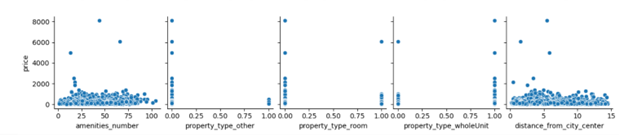
\includegraphics{outliers.png}
    \captionsetup{justification=centering}
    \captionof{figure}{Scatter plots showing outliers}
\end{center}
\vspace{.5cm}
\textbf{• Transforming skewed data}\\
I performed two important data transformations to improve the quality of the data and the performance of the models.\\ Firstly, I applied a log transformation to skewed data using the numpy log1p function. The skewed features were identified by their skewness value, which was calculated using the pandas skew function. Non boolean features with a skewness value greater than 1 or less than -1 were transformed. This transformation helps to normalize the distribution of the data and improve the accuracy of linear models.\\
Secondly, I applied a standard scaling to continuous data using the StandardScaler function from the Scikit-learn library. A list of continuous features was selected and scaled using the scaler.fit\textunderscore transform method. Scaling the data ensures that each feature has a similar range and mean, which is beneficial for models that rely on distance-based calculations, such as K-nearest neighbours and support vector machines.\\
To verify the impact of the log transformation, I plotted the distribution of the 'price' feature using the seaborn distplot function before and after the transformation. The initial distribution was positively skewd with a value of 19.677297, which can make it difficult for models to accurately predict high-priced listings. After the log transformation, the distribution became more normal, with a skewness value of 0.309012.
\begin{center}
    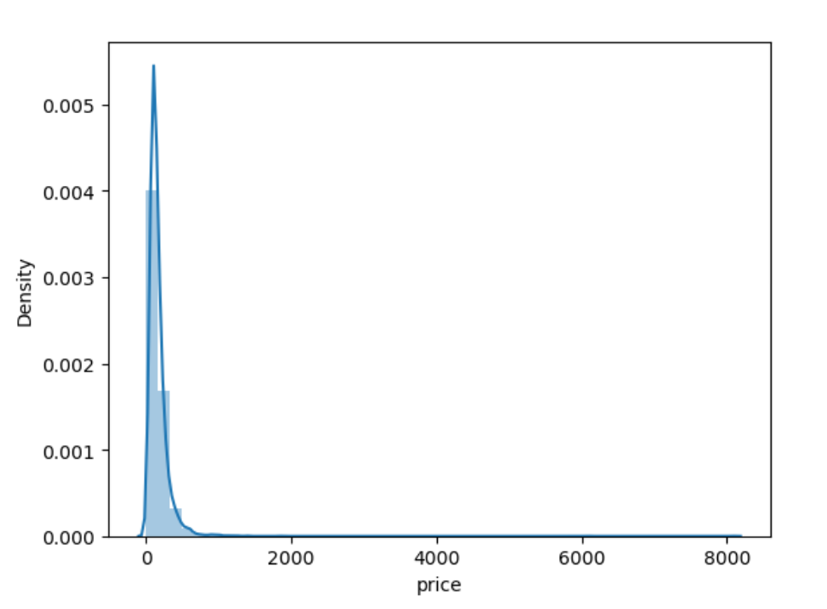
\includegraphics[width=0.7\textwidth,height=0.4\textheight]{price_before.png}
    \captionsetup{justification=centering}
    \captionof{figure}{Price distribution before log transformation}
\end{center}
\begin{center}
    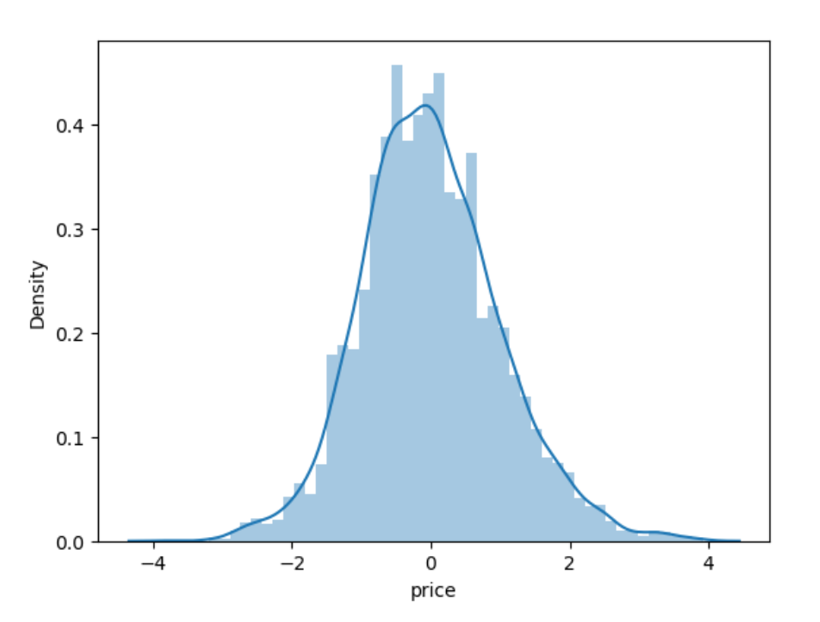
\includegraphics[width=0.7\textwidth,height=0.4\textheight]{price_after.png}
    \captionsetup{justification=centering}
    \captionof{figure}{Price distribution after log transformation}
\end{center}
\vspace{.5cm}
\textbf{• Dropping intercorrelated features}
As a result of observing the correlations between features using a heatmap, several features were identified as having a high correlation with other variables and were subsequently dropped. These features include 'host\textunderscore total\textunderscore listings\textunderscore count', 'calculated\textunderscore host\textunderscore listings\textunderscore count', 'availability\textunderscore 30', 'availability\textunderscore 60', 'availability\textunderscore 90', 'room\textunderscore type\textunderscore Private room', and 'property\textunderscore type\textunderscore room'. By removing these highly correlated features, I ensured that the model would not be influenced by redundant information and would instead focus on the most informative variables.\\
To explore the importance of the distance feature in predicting the price of a listing, a scatter plot was created to visualize the relationship between distance and price, with neighbourhood as the color of each point. The resulting plot showed a clear relationship between distance and price, with no discernible pattern based on neighbourhood color. This suggests that the distance feature may be sufficient for predicting price, and thus the neighbourhood feature may not be necessary for our analysis. To reflect this, the neighbourhood column was subsequently dropped from the dataframe using df.drop().

\begin{center}
    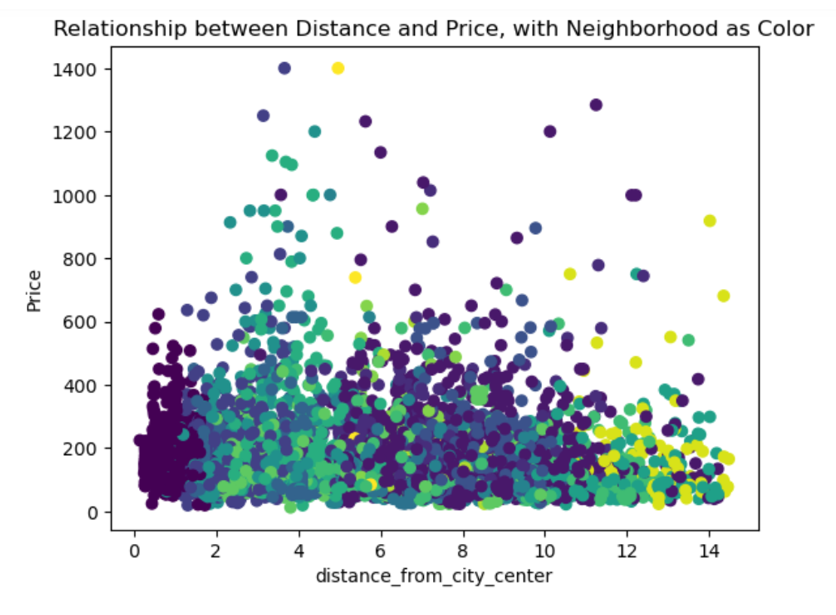
\includegraphics[width=0.9\textwidth,height=0.4\textheight]{distance_price.png}
    \captionsetup{justification=centering}
    \captionof{figure}{Relationship between distance from center and price, with neighbourhood as the color}
\end{center}

\section{Key Findings and Insights}
From our exploratory data analysis, I find that the most common property types are apartments, houses, and townhouses, and that the most expensive listings are usually located in the city center.\\
I also find that there is a strong positive correlation between the number of bedrooms and the price of the listing. 

\section{Formulating at least 3 hypothesis about this data}
After completing data cleaning and feature engineering, I conducted exploratory data analysis to gain insights into the data. I visualized the distribution of the target variable, price, and found that it was right-skewed, with a few extreme values. I also explored the relationships between the target variable and other features, using scatterplots, boxplots, and correlation matrices. I discovered that some features, such as the number of bedrooms, bathrooms, and accommodates, were strongly correlated with the price.\\
Based on these insights, I formulated three hypotheses about the data:\\
• Hypothesis 1: Units that are rented out as a whole tend to be more expensive.\\
• Hypothesis 2: Listings with more amenities tend to have higher prices.\\
• Hypothesis 3: Listings with a higher number of accommodates (the maximum number of guests that the listing can accommodate) tend to have higher prices.\\

\section{Conducting a formal significance test for one of the hypotheses and discuss the results}
A hypothesis test was conducted to determine if there is a significant difference in the mean price of whole units versus non-whole units. The data was split into two groups based on the property\textunderscore type\textunderscore wholeUnit column, and a two-sample t-test was performed assuming unequal variances.\\ 
The results showed a statistically significant difference in the mean price of the two groups, with a t-statistic of -68.16 and a p-value of 0. This indicates that the difference in the mean price between whole units and non-whole units is unlikely to have occurred by chance, and I can reject the null hypothesis that there is no difference in price between the two groups.\\ 

\section{Suggestions for next steps in analysing this data}
Next steps in analysing this data could include using machine learning algorithms to predict the price of listings based on various attributes or to identify factors that affect occupancy rates. I could also analyze the reviews data to identify common themes or sentiments among guest reviews and use these insights to improve the quality of listings.\\ Additionally, I could collect more data on external factors, such as weather or events in the city, and analyze their impact on the Airbnb market in Seattle.

\section{A paragraph that summarizes the quality of this data set and a request for additional data if needed}
The dataset used in this analysis is quite extensive, containing a total of 92 attributes in the listings file alone. The data covers a broad range of information related to both the listings and reviews of Airbnb in Seattle. To ensure the dataset was suitable for analysis, several data cleaning and feature engineering procedures were performed. \\
These included dropping non-relevant features, handling missing values, transforming data types, encoding categorical variables, and creating new features from existing ones. In cases where missing values existed, the medians were used as replacement values. However, for the "beds" feature, rows with missing values were removed. Many features underwent a data type transformation, and categorical features were encoded to numerical values for the purpose of analysis.\\
In order to provide a more comprehensive analysis, it would be useful to have additional data such as demographic information on Seattle neighbourhoods and data on actual occupancy rates of Airbnb listings in Seattle.



\end{document}